\chapter{Tervez\'es}\label{chapter:tervezes}
A tervezési folyamat elején alapvető fontosságú tisztázni, mit is szeretnénk létrehozni. Az itt bemutatásra kerülő alkalmazás egy videómegosztó és interaktív csevegési platform, amely lehetővé teszi a felhasználók számára, hogy videókat nézzenek, és osszanak meg barátaikkal, miközben élő csevegés során beszélgethetnek a videók tartalmáról. Az alkalmazás célja, hogy összekapcsolja az embereket, lehetővé téve számukra, hogy megosszák élményeiket és gondolataikat valós időben.


\section{Főbb funkciók}

\begin{enumerate}
  \item \textbf{Videómegtekintés:} A felhasználók széles körű videókat tekinthetnek meg, amelyek számos témát és érdeklődési kört fednek le, biztosítva, hogy mindenki találjon magának megfelelő tartalmat.
  
  \item \textbf{Élőcsevegés:} A platform lehetővé teszi a felhasználók számára, hogy valós idejű beszélgetéseket folytassanak, miközben videókat néznek, így közvetlen kommunikációt és interakciót biztosítva a közösségi élmény fokozása érdekében.
  
  \item \textbf{Szobák kezelése:} A felhasználók létrehozhatnak és kezelhetnek privát vagy nyilvános szobákat, ahol különleges érdeklődési körök vagy témák köré csoportosulhatnak, így személyre szabott közösségi tér alakítható ki.
  
  \item \textbf{Profil szerkesztés:} Minden felhasználó rendelkezik egy személyes profillal, amit testreszabhatnak, hogy kifejezzék személyiségüket, és megoszthassák érdeklődési köreiket.
  
  \item \textbf{Regisztráció/Bejelentkezés:} Az alkalmazás biztosít egy egyszerű és biztonságos regisztrációs és bejelentkezési folyamatot, lehetővé téve új felhasználók számára, hogy csatlakozzanak a közösséghez.
\end{enumerate}


\section{Átfogó struktúra}
A kliens-szerver-adatbázis struktúrát 3 rétegű topológiának nevezzük. A 3-rétegű architektúra előnye, hogy modularizálja az alkalmazás kódját, ami megkönnyíti a karbantartást, a tesztelést és a skálázhatóságot.
\begin{figure}[H]
    \centering
    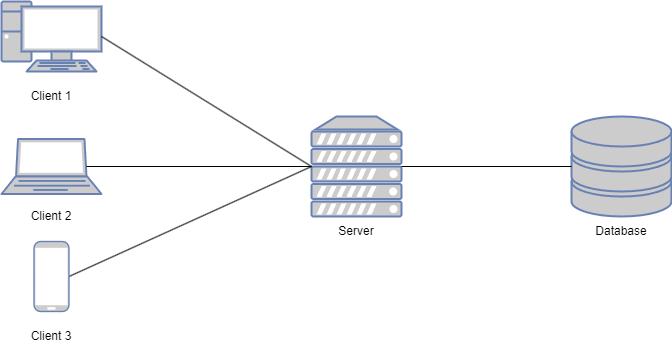
\includegraphics[width=14.0truecm]{images/Client-Server-DB.png}
    \caption[Kliens-Szerver-Adatbázis struktúra]{Kliens-Szerver-Adatbázis struktúra}
    \label{fig:architecture}
\end{figure}
\subsection{Kliens réteg}
A kliens oldal felelős a felhasználói interakciókért és a felhasználói felület megjelenítéséért. Itt találhatók a gombok, formok, és egyéb elemek, amikkel a felhasználók közvetlenül érintkeznek. A kliens oldalon futó kód gyakran aszinkron módon kommunikál a szerverrel, hogy adatokat kérjen vagy küldjön.
\\
\subsection{Szerver réteg}
A szerver oldal felelős a kliens oldal által küldött kérések feldolgozásáért, és a válaszok generálásáért. Itt található az üzleti logika, és az adatbázis kezelés. A szerver oldali kód futása általában szinkron módon történik, és a kliens oldali kérések feldolgozása után küldi a válaszokat.

\subsection*{Adatbázis réteg}
Ez a réteg tárolja az alkalmazás állapotát és adatát. Gyakran SQL (pl. MySQL, PostgreSQL) vagy NoSQL (pl. MongoDB) adatbázisokat használnak itt.

\section{Kliens oldali logika}
A kliens oldali logika szigorú hierarchikus struktúra foglalja magába. Az alkalmazáson belüli komponensek mind horizontálisan, mind vertikálisan szerveződnek.
\begin{figure}[H]
    \centering
    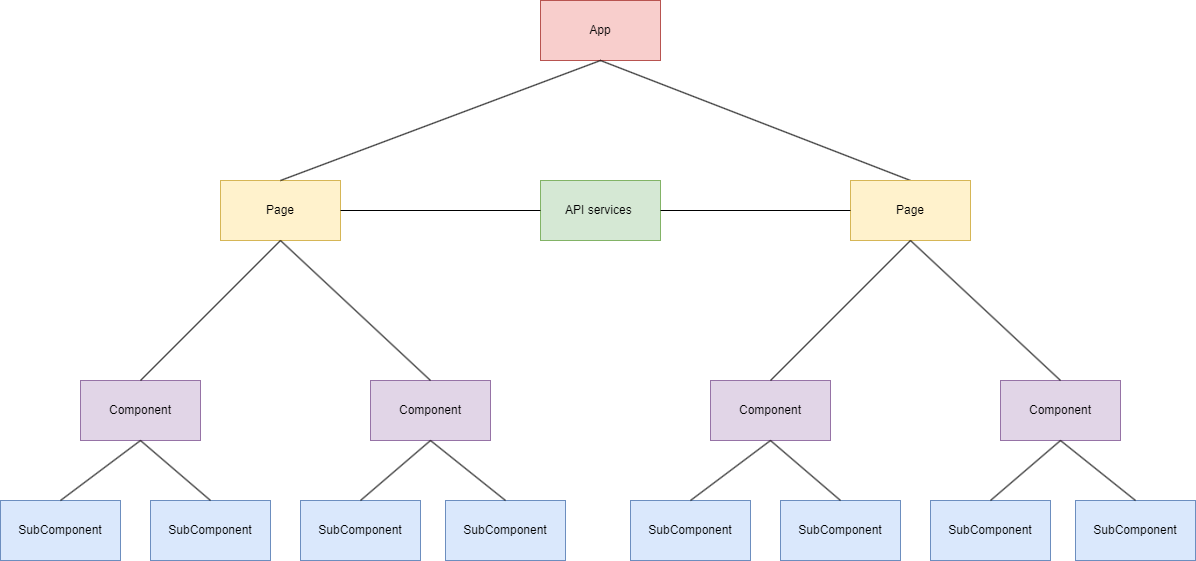
\includegraphics[width=14.0truecm]{images/Frontend_architecture.png}
    \caption{Frontend Architektúra}
    \label{fig:frontend_architecture}
\end{figure}
A fejlesztés során az egyik fő szempont a komponensek újrafelhasználhatósága, kód strukturáltsága volt.
\\
\textbf{A komponensek főbb tulajdonságait:}
\begin{itemize}
    \item \textbf{App:} Az alkalmazás gyökér komponense. Itt található a Router, amely a különböző útvonalakhoz rendeli a megfelelő komponenseket.
    \item \textbf{Page:} Az alkalmazás View komponensei. A különböző oldalakat reprezentálják. Itt találhatóak a különböző komponensek, amelyek a megjelenítést végzik. Illetve itt használom az API hívásokat is.
    \item \textbf{API services:} Itt találhatóak a különböző API végpontokat kezelő függvények.
    \item \textbf{Component:} Az alkalmazás nagyobb komponensei. Ezek a komponensek több kisebb komponensből állnak össze.
    \item \textbf{SubComponent:} Az alkalmazás kisebb komponensei. Ezek a komponensek csak egy adott feladatot látnak el.
\end{itemize}


\section{Szerver oldali logika}
\subsection{Architektúra}
Az alkalmazásnál MVC (Model-View-Controller) architektúrára építettem, illetve
bővítettem a Repository és a Service rétegekkel. Az MVC architektúra egy
architektúrális minta, amely a felhasználói felületet (View), az alkalmazás
logikáját (Controller) és az adatokat (Model) három különálló részre osztja.
A Repository réteg a Model réteghez tartozik, a Service réteg pedig a Controller réteghez.
A további bontást a felelősségi körök elkülönítése, kód átláthatóságának növelése, a bővíthetőség és a tesztelhetőség indokolta.
\\
\\
\begin{figure}[H]
    \centering
    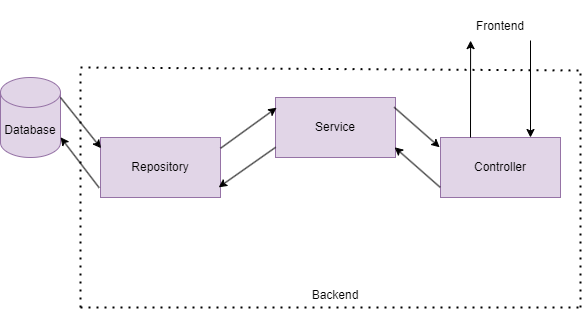
\includegraphics[width=14.0truecm]{images/Backend_architecture.png}
    \caption{Backend Architektúra}
    \label{fig:backend_architecture}
\end{figure}
\textbf{A rétegek főbb tulajdonságait:}
\begin{itemize}
    \item \textbf{Adatbázis}: Az alkalmazás adattára. Itt tárolódnak a statikus és dinamikus adatok.
    \item \textbf{Repositoryk}: Az adatbázis és az alkalmazás logikája közötti köztes réteg. CRUD műveletek, komplex lekérdezések.
    \item \textbf{Servicek}: Az üzleti logika helye. Itt történnek a komplex számítások, validációk és egyéb logikai műveletek.
    \item \textbf{Controllerek}: Az API végpontokat kezelő réteg. Fogadják a kliens kéréseit, és válaszokat generálnak.
\end{itemize}

\section{Adatbázis}
\subsection{ER modell egyedei és tulajdonságai}
Az alkalmazás működésének alapját az entitások és azok közötti kapcsolatok adják, amelyek elengedhetetlenek a program struktúrájában. A következő entitások kiemelkedő szerepet töltenek be:

\begin{itemize}
    \item \textbf{Felhasználók (Users):} Kapcsolatban állnak a képekkel (\textit{Images}) és a szobákkal (\textit{Rooms}), ezáltal teremtve meg a közösségi interakció alapjait.
    \item \textbf{Szobák (Rooms):} Összekötik a felhasználókat a videókkal (\textit{Videos}), lehetővé téve számukra, hogy tematikusan csoportosuljanak és megosszák videóikat.
\end{itemize}

Ezen entitások közötti kapcsolatok biztosítják a platform dinamikus és interaktív jellegét, ahol a felhasználók egymással és a tartalommal kölcsönhatásba lépnek.
\vspace{7em}
\\
\textbf{User-ek tulajdonságai:}
\begin{itemize}
    \item \texttt{Id}: Elsődleges kulcs, Guid típusú.
    \item \texttt{Name}: Felhasználó neve, szöveg típusú.
    \item \texttt{Email}: Felhasználó email címe, szöveg típusú.
    \item \texttt{PasswordHash}: Felhasználó jelszavának hash-elt változata, szöveg típusú.
    \item \texttt{Salt}: Felhasználó jelszavának sója, szöveg típusú.
    \item \texttt{BirthDate}: Felhasználó születési dátuma, dátum típusú.
\end{itemize}
\textbf{Image-ek tulajdonságai:}
\begin{itemize}
    \item \texttt{Id}: Elsődleges kulcs, Guid típusú.
    \item \texttt{Data}: Kép binárisa, byte tömb típusú.
\end{itemize}
\textbf{Room-ok tulajdonságai:}
\begin{itemize}
    \item \texttt{Id}: Elsődleges kulcs, Guid típusú.
    \item \texttt{Name}: Szoba neve, szöveg típusú.
    \item \texttt{CreatorId}: Tulajdonos azonosítója, Guid típusú.
    \item \texttt{CreationTime}: Szoba létrehozásának ideje, dátum típusú.
    \item \texttt{CurrentVideoId}: Jelenleg lejátszott videó azonosítója, Guid típusú.
    \item \texttt{PasswordHash}: Szoba jelszavának hash-elt változata, szöveg típusú.
    \item \texttt{Salt}: Szoba jelszavának sója, szöveg típusú.
\end{itemize}
\textbf{Video-k tulajdonságai:}
\begin{itemize}
    \item \texttt{Id}: Elsődleges kulcs, Guid típusú.
    \item \texttt{Title}: Videó címe, szöveg típusú.
    \item \texttt{Url}: Videó URL-je, szöveg típusú.
    \item \texttt{ThumbnailURL}: Videó thumbnail-je, szöveg típusú.
\end{itemize}

\begin{figure}[H]
    \centering
    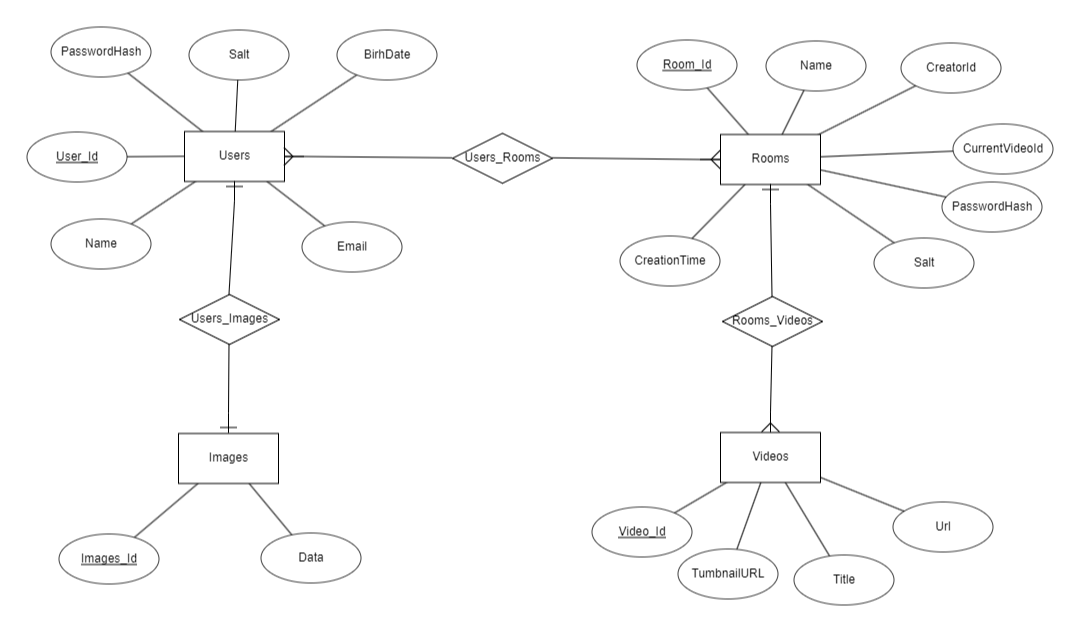
\includegraphics[width=15.0truecm]{images/er_modell.png}
    \caption{ER modell}
    \label{fig:er_modell}
\end{figure}

\subsection{Relációs modell}
\textbf{Az egyedek közötti kapcsolatok:}
\begin{itemize}
    \item \texttt{Users-Images}: 1:1 Egy felhasználóhoz tartozhat egy kép, és a kép csak egy fel-
          használóhoz.
    \item \texttt{Users-Rooms}: N:N Egy felhasználóhoz tartozhat több szoba, egy szoba is tartozhat
          több felhasználóhoz.
    \item \texttt{Room-Video}: 1:N Egy szobához tartozhat több videó, de egy videó csak egy
          szobához tartozhat.
\end{itemize}

\begin{figure}[H]
    \centering
    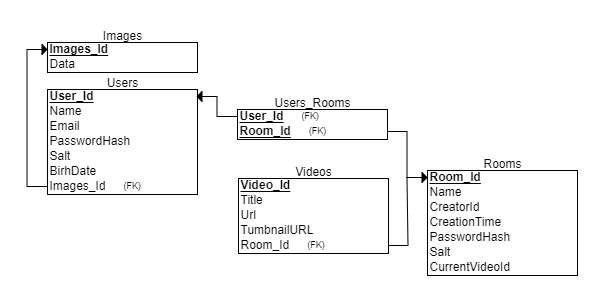
\includegraphics[width=15.0truecm]{images/relation_modell.png}
    \caption{Relációs modell}
    \label{fig:relation_modell}
\end{figure}

\subsection{Szoftvertervezési elvek}
A szoftvertervezési elvek alapvető útmutatások a kiváló kód fejlesztéséhez. Ezek az iránymutatások növelik a kód minőségét, gyorsítják a fejlesztési folyamatot és minimalizálják a hibalehetőségeket. Az ilyen elvek segítenek abban, hogy a kód könnyen újrafelhasználható és karbantartható legyen.

A kód olvashatóságát és tesztelhetőségét is javítják, ami hosszú távon időt és erőforrást spórol. A rugalmasság és a bővíthetőség is nő, tehát a kód könnyen adaptálható új funkciók vagy változások esetén. Továbbá, ezek az elvek ösztönzést nyújtanak a kódbázis redundancia kiküzsöbölésére, amely csökkenti a komplexitást és növeli a kohéziót. Az elvek célja a kód moduláris felépítése és az alacsonyabb összekapcsoltság, ami hozzájárul a jobb szervezettséghez és könnyebb karbantartáshoz.

Összességében, a szoftvertervezési elvek olyan iránymutatások, amelyek célja a hatékony, karbantartható és minőségi kód létrehozása.
A szoftver implementációja során a SOLID elveket vettem alapul.

\section{UML diagram}

\begin{figure}[H]
    \centering
    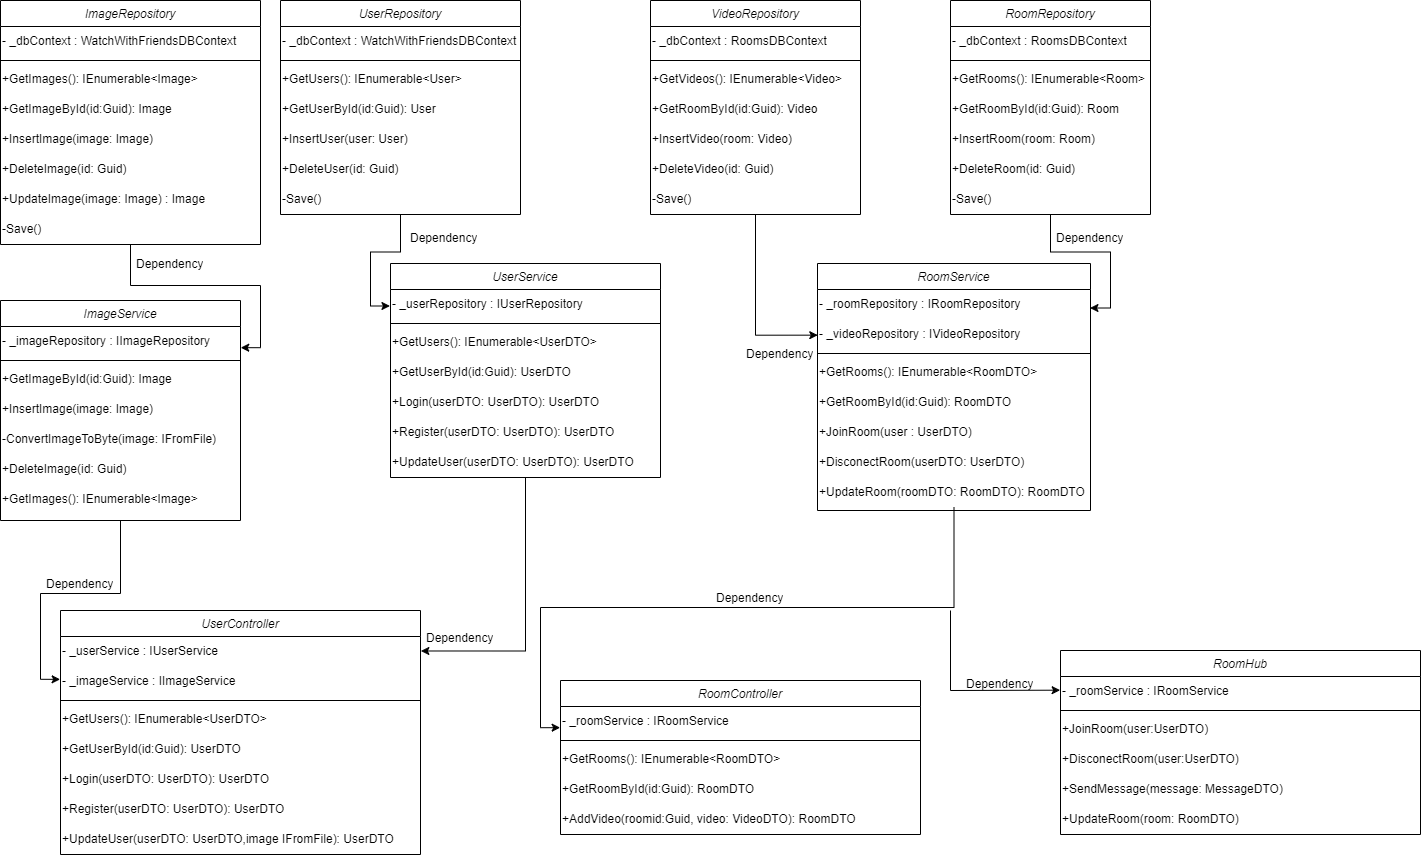
\includegraphics[width=14.0truecm]{images/UML_Diagram.png}
    \caption{UML Diagram}
    \label{fig:uml_diagram}
\end{figure}

Az architektúra alapját egy kibővített MVC (Model-View-Controller) rendszer adja,
amely kifinomult kapcsolatokat biztosít az egyes szerveroldali osztályok között. Mivel a back-end és a front-end kapcsolata indirekt, ezért a megjelenítési oldalon található logika nincs semmilyen ráhatással a szerver struktúrális felépítésére.
Ebben az elrendezésben az egyes osztályok nem csak az alapvető CRUD (Create, Read, Update, Delete) műveletekért felelnek, hanem a komplex üzleti logika egyedi implementációját is lehetővé teszik. Az adatmodell és a kontroller között az adatátviteli objektumok (DTO-k) és a repository minták segítenek a moduláris és tiszta kód struktúra fenntartásában. A repository-k pedig közvetlenül a dedikált adatbázis-kontextusokhoz kapcsolódnak.

A kapcsolatok közötti szoros integráció lehetővé teszi az adatok egyszerű és következetes kezelését, miközben fenntartja a kód karbantarthatóságát és tesztelhetőségét. Az egész rendszer ezen az elrendezésen alapul, így garantálva, hogy a szerveroldali logika
jól szervezett és hatékony maradjon.
